\documentclass[12pt]{beamer}
\usepackage[utf8]{inputenc}
\usepackage{lmodern}
\usepackage{german}
\usetheme{Berkeley}
\title[Design-Review Semesterarbeit]{Implementation einer Win/Win Strategie für das TSP}
\author{Andreas Brönnimann}
\institute{ZHAW - Zürcher Hochschule für Angewandte Wissenschaften}
\date{30.01.2012}

\setbeamerfont{footnote}{size=\tiny}
\setbeamertemplate{footline}[frame number]
\setbeamertemplate{navigation symbols}{}

\begin{document}

    \begin{frame}
        \titlepage
    \end{frame}

    \begin{frame}
        \frametitle{Ablauf}
        \tableofcontents
    \end{frame}

    \section{Stand der Arbeit}
    \begin{frame}
        \frametitle{Stand der Arbeit}
	    \begin{itemize}
                \item Algorithmus implementiert
                \item Implementation wird getestet
                \item Erste Auswertungen gemacht
                \item Struktur Dokumentation erstellt
                \item Dokumentation begonnen
            \end{itemize}
    \end{frame}

    \section{Beispiel}
    \begin{frame}
    \frametitle{Beispiel}
        \begin{figure}[H]
	    \centering
	        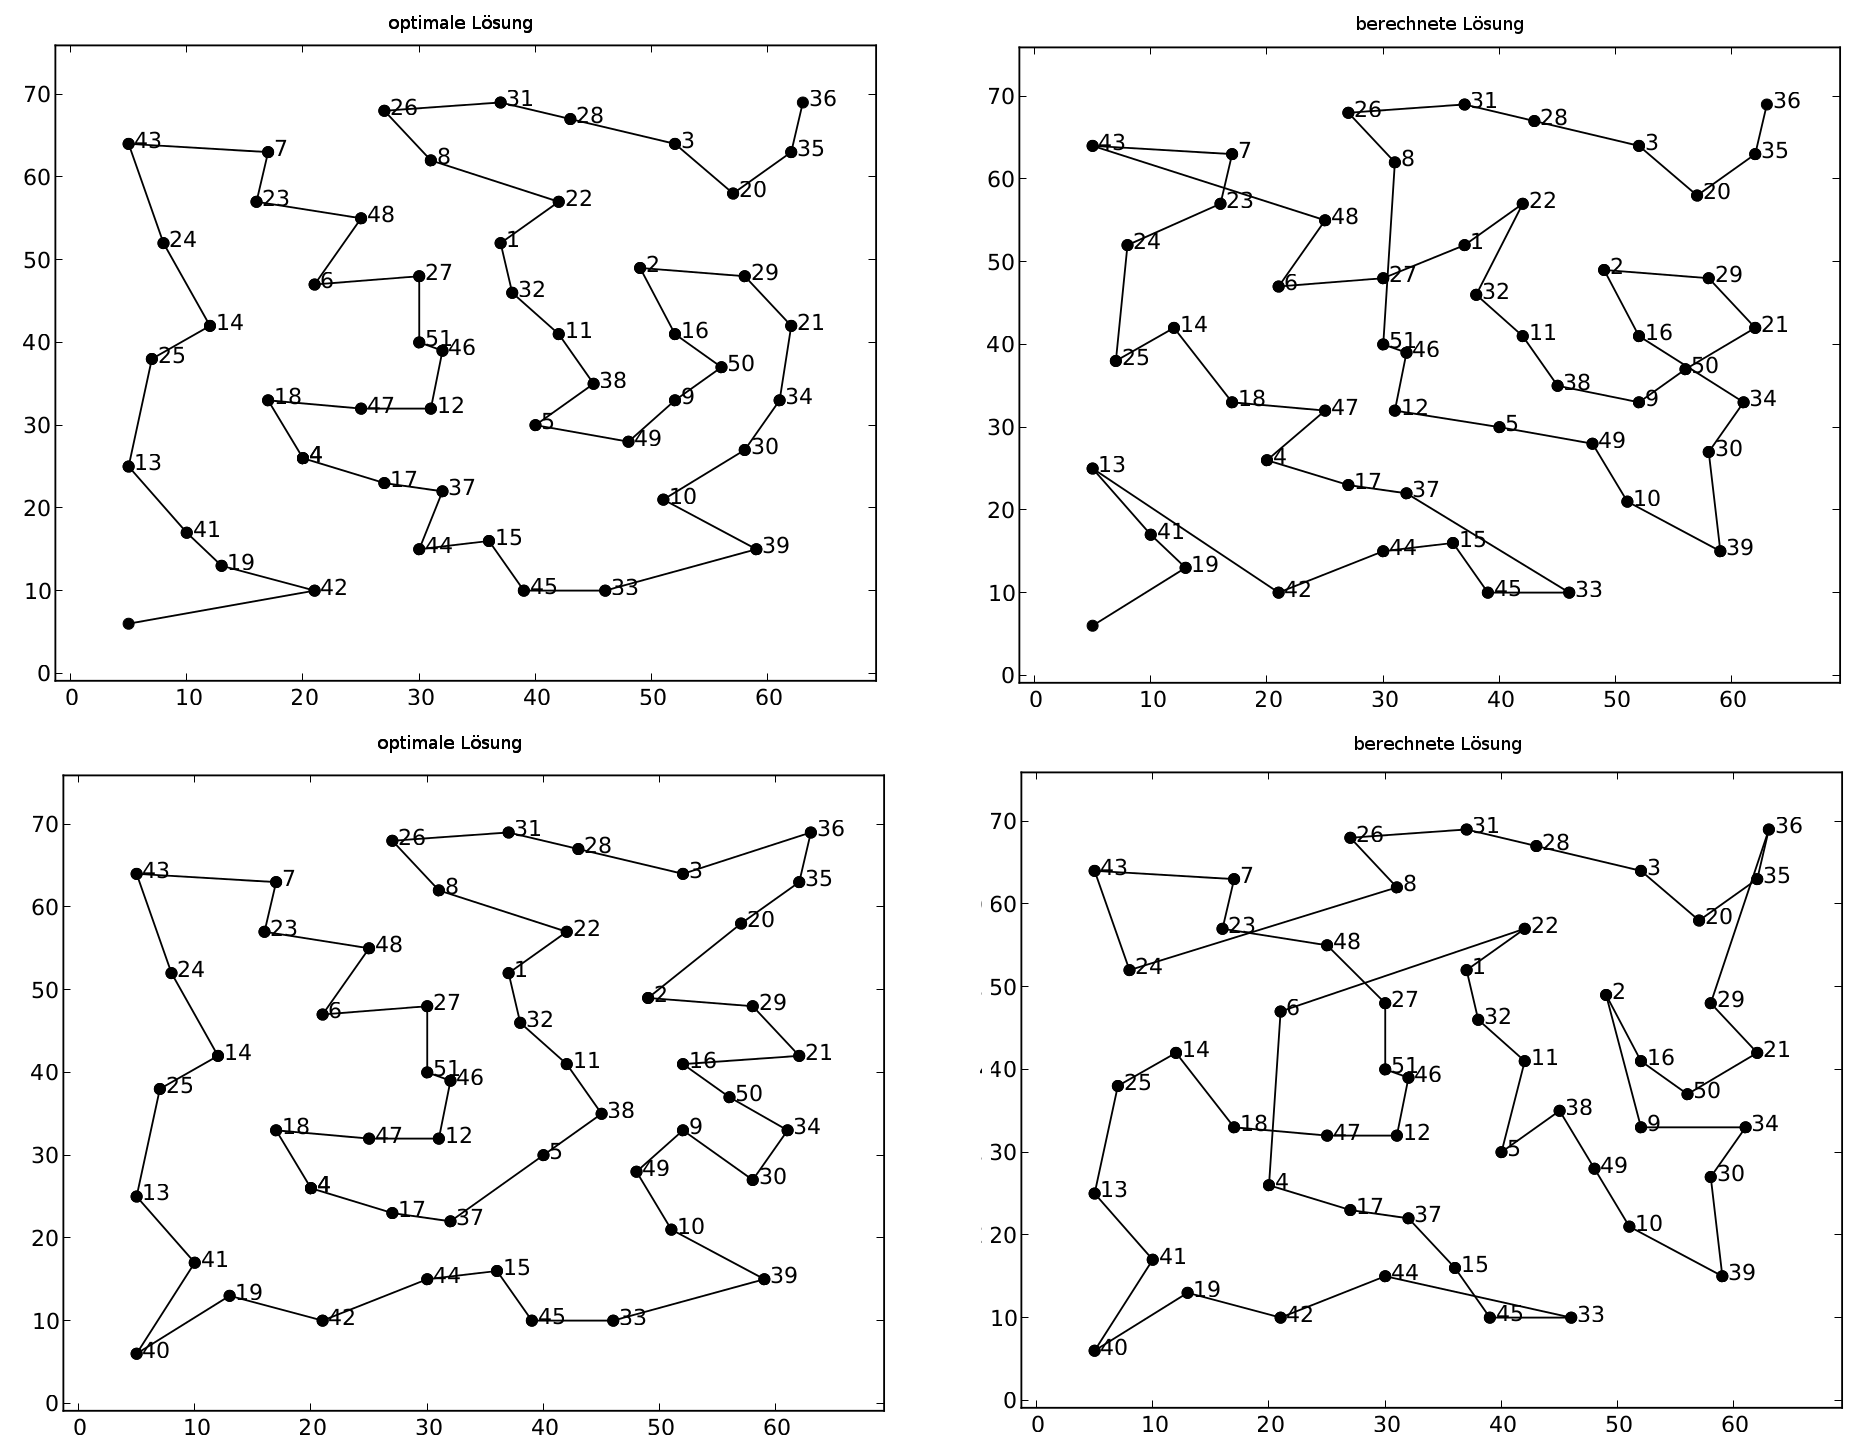
\includegraphics[width=9cm]{gfx/eil51_comparison}
        \end{figure}
    \end{frame}

    \begin{frame}
        \frametitle{Beispiel}
	    \begin{itemize}
                \item TSP: Weg 15\% schlechter als das Optimum
                \item HPP: Weg 14\% schlechter als das Optimum
                \item Kaum unterschiede zwischen TSP und HPP
            \end{itemize}
    \end{frame}

    \begin{frame}
    \frametitle{Beispiel}
        \begin{figure}[H]
	    \centering
	        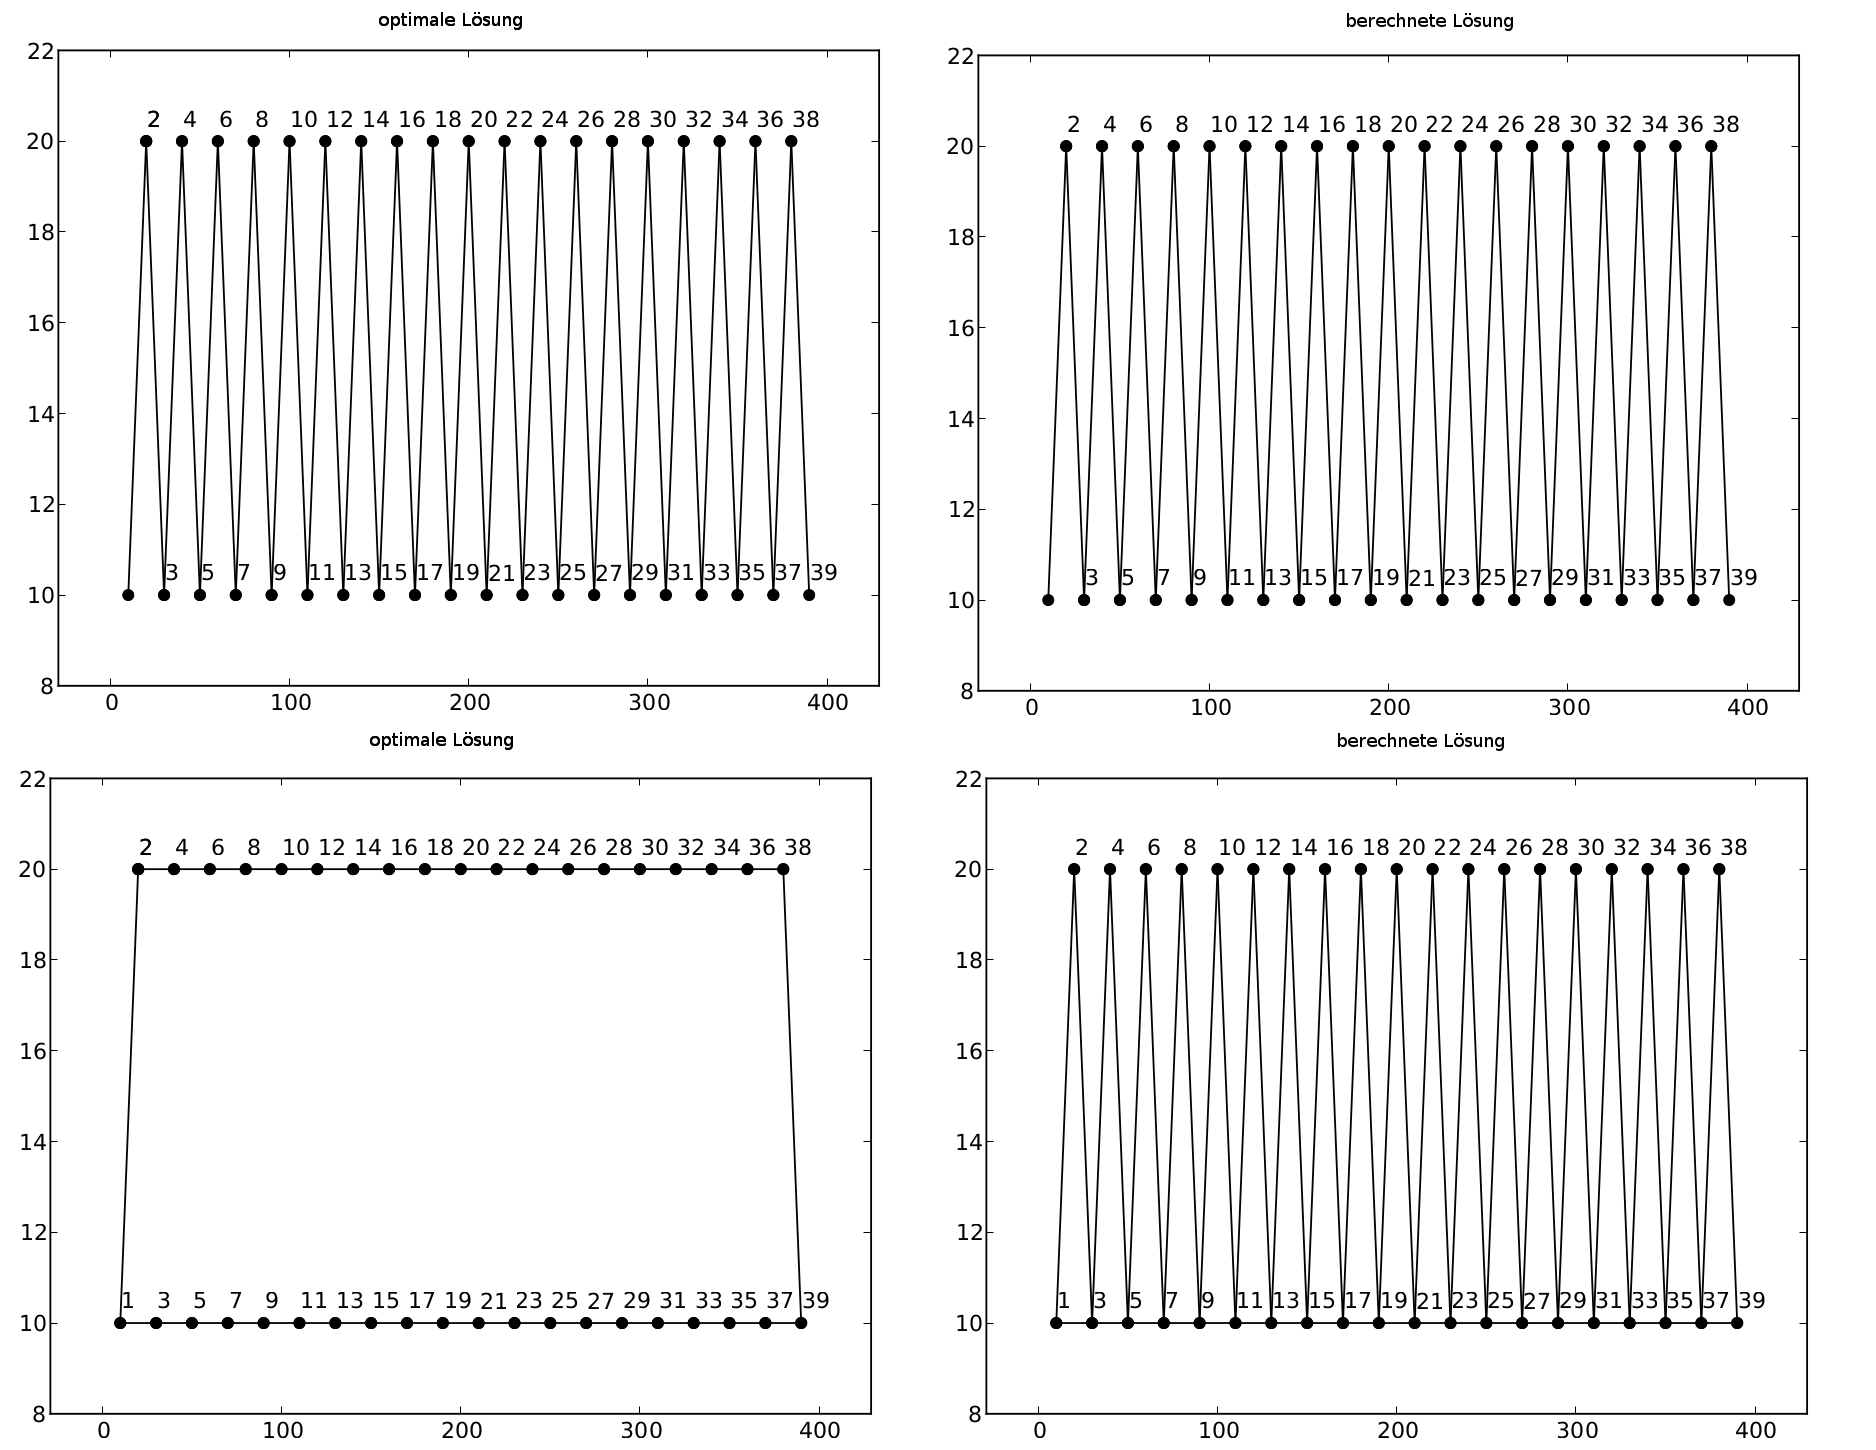
\includegraphics[width=9cm]{gfx/zz_comparison}
        \end{figure}
    \end{frame}

    \begin{frame}
        \frametitle{Beispiel}
	    \begin{itemize}
                \item TSP: Weg 6\% schlechter als das Optimum
                \item HPP: Weg 1\% schlechter als das Optimum
                \item HPP ist TSP überlegen
            \end{itemize}
    \end{frame}

    \section{Vorgehen}
    \begin{frame}
        \frametitle{Vorgehen}
	    \begin{itemize}
                \item Berechnung exakte Lösung mit Concorde für TSP
                \item Einfügen einer Dummy-City (Distanz 0 zu allen Städten)
                \item Berechnung exakte Lösung mit Concorde für HPP
                \item Beginn und Ende der Route werden als s und t verwendet
                \item Berechnung der Lösung mittels eigener Implementation
            \end{itemize}
    \end{frame}

    \section{Weitere Planung}
    \begin{frame}
        \frametitle{Geplante Auswertungen}
	    \begin{itemize}
                \item Beschreibung Win/Win
                \item Dokumentation Algorithmen
                \item Benchmarks TSPLIB
                \item Benchmarks generierte Probleme
            \end{itemize}
    \end{frame}

    \section{Fragen}
    \begin{frame}
    \frametitle{Fragen}
        \begin{figure}[H]
	    \centering
	        
\includegraphics[width=6cm]{gfx/questionmark}
        \end{figure}
    \end{frame}
\end{document}
